\documentclass[tikz,border=8pt]{standalone}
\usepackage{amsmath}
\usetikzlibrary{arrows.meta,calc}

\definecolor{ink}{HTML}{21352F}
\definecolor{teal}{HTML}{087F7B}
\definecolor{blue}{HTML}{4B77A8}
\definecolor{gold}{HTML}{C58B2A}
\definecolor{rose}{HTML}{B65A62}

\begin{document}
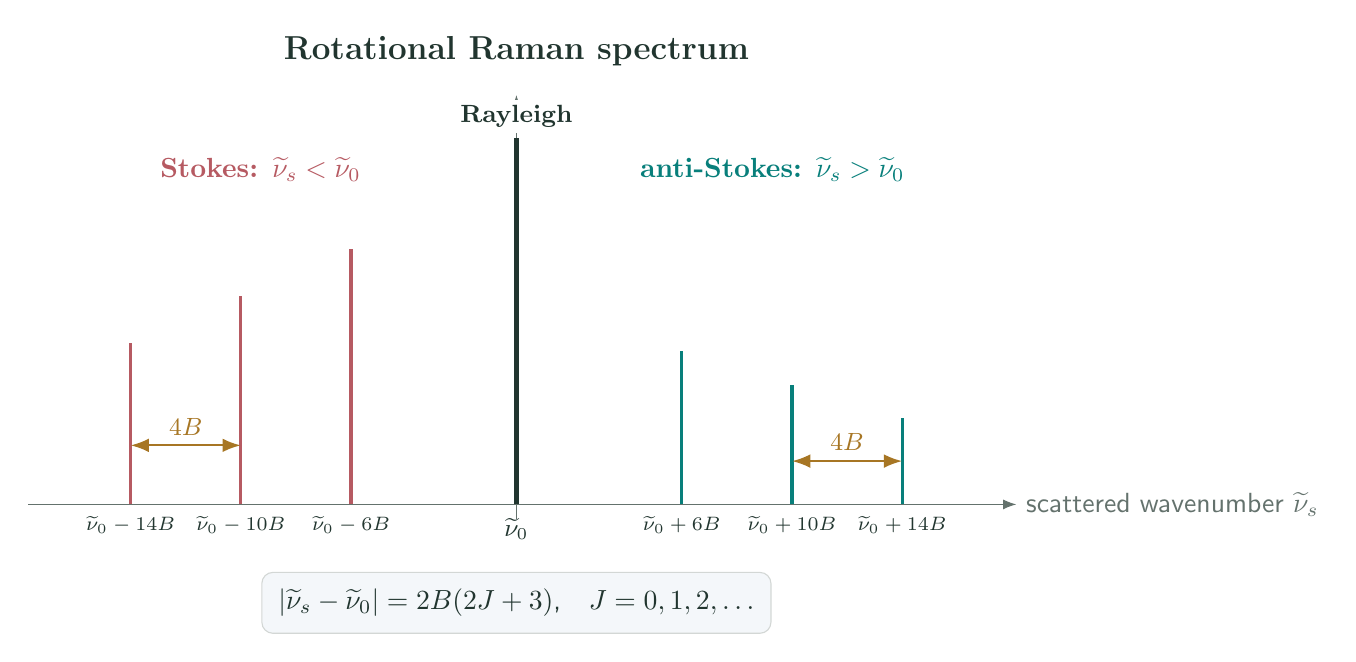
\begin{tikzpicture}[font=\sffamily,text=ink,>=Latex,x=1cm,y=1cm]
  \node[font=\bfseries\large] at (0,5.75)
    {Rotational Raman spectrum};
  \draw[->,ink!70] (-6.2,0)--(6.35,0)
    node[right] {scattered wavenumber $\widetilde\nu_s$};
  \draw[->,ink!70] (0,-.18)--(0,5.2);
  \node[below,font=\small] at (0,-.06) {$\widetilde\nu_0$};

  % Rayleigh line
  \draw[ink,ultra thick] (0,0)--(0,4.65);
  \node[font=\small\bfseries,fill=white,inner sep=2pt]
    at (0,4.93) {Rayleigh};

  % Stokes shifts -(6B,10B,14B), represented on a uniform 4B scale.
  \foreach \x/\h/\lab in {-2.1/3.25/6B,-3.5/2.65/10B,-4.9/2.05/14B}{
    \draw[rose,very thick] (\x,0)--(\x,\h);
    \node[below,font=\scriptsize] at (\x,-.03)
      {$\widetilde\nu_0-\lab$};
  }
  % Anti-Stokes shifts +(6B,10B,14B), lower thermal intensity.
  \foreach \x/\h/\lab in {2.1/1.95/6B,3.5/1.52/10B,4.9/1.10/14B}{
    \draw[teal,very thick] (\x,0)--(\x,\h);
    \node[below,font=\scriptsize] at (\x,-.03)
      {$\widetilde\nu_0+\lab$};
  }

  \node[rose,font=\bfseries] at (-3.25,4.25)
    {Stokes: $\widetilde\nu_s<\widetilde\nu_0$};
  \node[teal,font=\bfseries] at (3.25,4.25)
    {anti-Stokes: $\widetilde\nu_s>\widetilde\nu_0$};

  \draw[<->,gold!85!black,thick]
    (-4.90,.75)--(-3.50,.75)
    node[midway,above,font=\small] {$4B$};
  \draw[<->,gold!85!black,thick]
    (3.50,.55)--(4.90,.55)
    node[midway,above,font=\small] {$4B$};

  \node[draw=ink!20,fill=blue!6,rounded corners=4pt,
        align=center,inner sep=6pt] at (0,-1.25)
    {$|\widetilde\nu_s-\widetilde\nu_0|
      =2B(2J+3)$,\quad $J=0,1,2,\ldots$};
\end{tikzpicture}
\end{document}
